\subsection{Проверка инвариантов}

Задача model checker-а – проверка пользовательских инвариантов во всех достижимых состояниях системы. Пользователь задает инвариант через реализацию интерфейса IPredicate (рис.~\ref{fig:predicate}). IPredicate предоставляет методы сигнала об ошибке Fail, добавления нового непрозрачного состояния Report, проверки корректности предиката IsCorrect и проверки на полноту отчета MakesSense.

\begin{figure}[h]
    \centering
    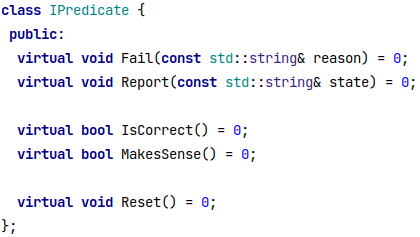
\includegraphics[width=0.75\textwidth]{img/predicate.png}
    \caption{Интерфейс предиката}
    \label{fig:predicate}
\end{figure}

Метод Fail в простейшем случае выполняет роль assert-а. Пользовательский код может просигнализировать таким образом о нарушении инварианта.

Метод Report – добавление нового непрозрачного состояния, которое может интерпретировать только реализация предиката. Такая функция нужна для того, чтобы проверять инварианты не только в каждой вершине, но и на всем пути исполнения в графе конфигураций. К примеру, мы можем с помощью этого механизма выстраивать порядок, в котором операции Set и Get завершались в atomic key value storage. Дальше можно, используя знание о причинности начала операций, написать проверку на линеаризуемость полученной истории.

Проверка корректности IsCorrect нужна по очевидным причинам. Проверка MakesSense на полноту отчета нужна, так как мы хотим иногда ограничивать глубину рассматриваемых исполнений, и это способ снятия метрики количества таких ветвей, чья длина начала превышать лимит, и мы перестали их дальше исполнять.

Мелкой деталью является функция сброса состояния предиката, которую подразумевается использовать при перезапуске системы.
